% --
% raw audio

\section{Raw Audio Waveforms}\label{sec:signal_raw}
\thesisStateReady
Physical acoustic waves are recorded by microphones, translating mechanical vibrations to electrical signals. 
Those electrical signals are further stored in \emph{waveform files} or \emph{audio files} with a specific audio format, for example the \texttt{.wav} format.
Apart from any compression technique the most important storage details are the bit resolution, for example \SI{24}{\bit} floating point and the sample rate $f_s$. 
%The sample rate defines, which frequency range of the continuous acoustic waveform is possible to store in a discrete representation.
The sample rate defines, which frequency range of a continuous acoustic waveform can be stored in a discrete representation.
This is restricted by the Nyquist-Shannon sampling theorem, where the maximal frequency of the signal $f_{x_{max}}$ should not exceed the half of the sampling frequency: 
\begin{equation}\label{eq:signal_raw_nyquist}
  f_{x_{max}} < \frac{fs}{2}
\end{equation}
to prevent aliasing effects.
That is the reason, why the compact disc (CD) format has a sampling frequency of \SI{44.1}{\kilo\hertz} resulting in a maximum signal frequency of \SI{22.05}{\kilo\hertz}, using the fact that humans do not hear above \SI{20}{\kilo\hertz} frequencies.
However it is also possible to go far beyond those \SI{44.1}{\kilo\hertz}, for instance used in telephone systems, where the sampling rate is \SI{8}{\kilo\hertz}.
It is possible to reduce the sampling rate, because voice does not need such a high sampling frequency to have sufficient quality and being understandable.
Music on the other hand requires a high sampling frequency for being enjoyable to listen to.

With the sampling frequency known, a discrete time signal of an audio recording $x \in \R^n$ can be expressed in vector notation:
\begin{equation}\label{eq:signal_raw_x}
  x = [x_1,\, x_2,\, \dots,\, x_n]^T
\end{equation}
with a total number of $n$ samples.
The recorded audio files provided in the speech command dataset \cite{Warden2018} used for the experiments in \rsec{exp}, are sampled with a sampling rate of \SI{16}{\kilo\hertz}, which is enough for human speech signals.
Further those recordings usually have a time duration of \SI{1}{\second}, apart from some individual shorter files.

For evaluation and visualization purpose, the author of this thesis recorded his own examples of the speech commands \{\enquote{left}, \enquote{right}, \enquote{up}, \enquote{down}, \enquote{go}\}.
Those showcase examples represent for instance actions in a video game and need to be feature extracted before they are classified with a neural network.
The example are shown in \rfig{signal_raw_showcase} in raw audio format.
\begin{figure}[!ht]
  \centering
    \subfigure[left]{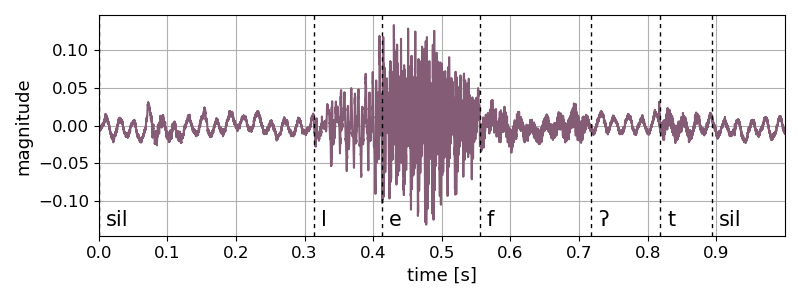
\includegraphics[width=0.45\textwidth]{./3_signal/figs/signal_raw_showcase_left0}}
    \subfigure[right]{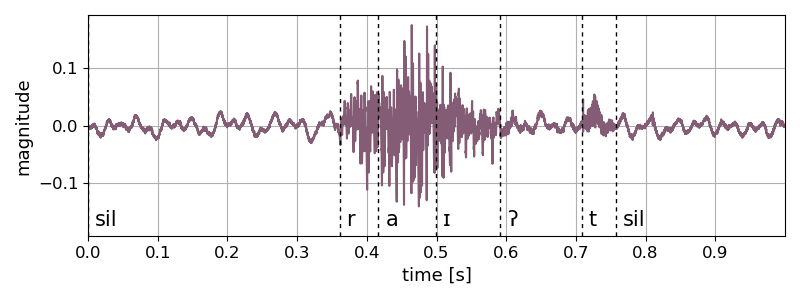
\includegraphics[width=0.45\textwidth]{./3_signal/figs/signal_raw_showcase_right0}}
    \subfigure[up]{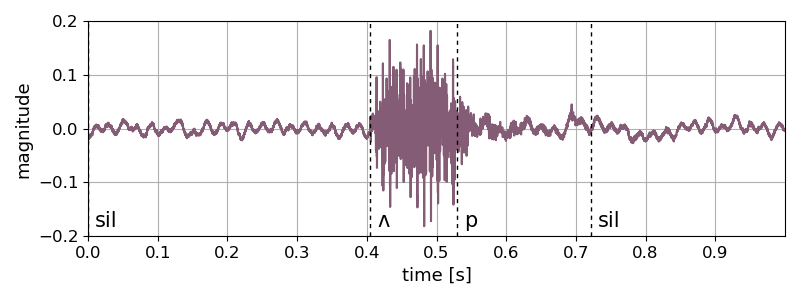
\includegraphics[width=0.45\textwidth]{./3_signal/figs/signal_raw_showcase_up0}}
    \subfigure[down]{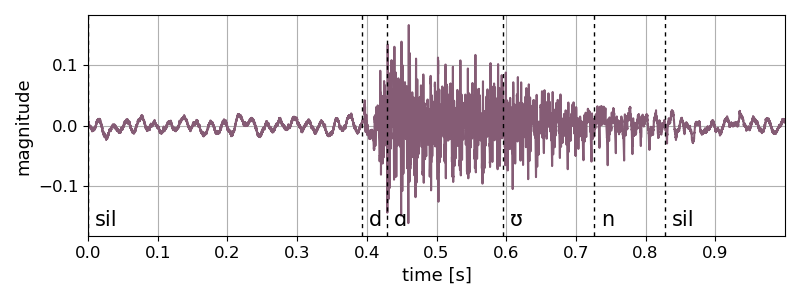
\includegraphics[width=0.45\textwidth]{./3_signal/figs/signal_raw_showcase_down0}}
    \subfigure[go]{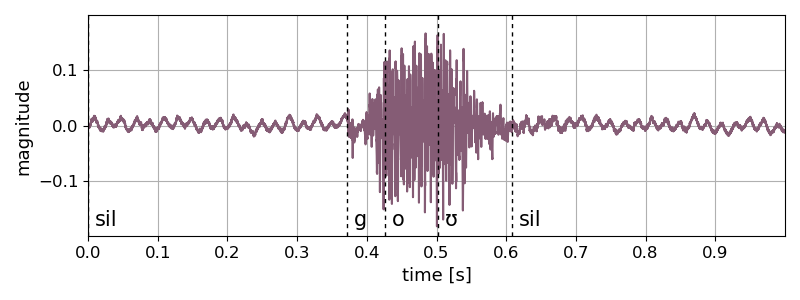
\includegraphics[width=0.45\textwidth]{./3_signal/figs/signal_raw_showcase_go0}}
  \caption{Raw audio waveform files, recorded by the author of this thesis with a simple consumer lavalier microphone.}
  \label{fig:signal_raw_showcase}
\end{figure}
\FloatBarrier
\noindent
From the shown raw audio files, one can estimate how long a speech command may take in terms of duration and see that usually a whole second is too much for a single speech command.
The pronunciation of words can of course deviate strongly in duration, but usually when commanding something it is preferred to speak short and well pronounced.
If a time interval of \SI{500}{\milli\second} is used to capture a speech command (this time interval is used in the feature extraction), it might happen that not every phoneme of the spoken words are captured. 
Often this might occur for words with glottal stops before consonants, for example the phoneme \enquote{t} in \enquote{left} or \enquote{right}, therefore the input features may only contain information of the first phonemes \enquote{lef} or \enquote{righ}.
But since Key Word Spotting (KWS) is restricted in its vocabulary and no similar words are contained within, it should be no problem in distinguishing those.

Another important aspect is to detect the onset position of the speech commands on the time axis. 
It is easy to see in \rfig{signal_raw_showcase} where the spoken words are beginning and ending, but usually not all recordings are as clean as those.
There might be a huge noise level or background noise or cut off signals, so that the detection of the right onset position for the \SI{500}{\milli\second} time interval within the \SI{1}{\second} recordings is not always appropriate.
An intuitive method is to simply use the signal energy to determine the onset of the key words.
If the signal $x \in \R^n$ is windowed with the length of a \SI{500}{\milli\second} striding frame with sample length $N$ of the window, the energy of each windowed signal is calculated as:
\begin{equation}
  e_{w}(m) = \sum_{i=0}^{N-1} \abs{x[i + m]}^2
\end{equation}
with shift index $m \in \mathcal{M} = \{0, 1, \dots, n - N + 1\}$, where $n$ is the total number of samples of $x$.
The onset sample number $o \in \mathcal{M}$ with the highest energy region can be determined by
\begin{equation}
  o = \underset{m \in \mathcal{M}}{\arg \max} \, e_{w}(m)
\end{equation}
for all windowed signal energies $e_{w}(m)$.

At last it should be noted, that the value range in the y-axis of audio recordings strongly depends on the microphone, amplifiers and post processing.
Therefore it is strongly recommended to normalize all recordings to a defined value range, with for instance the infinity norm:
\begin{equation}
  \hat{x} = \frac{x}{\norm{x}_\infty}
\end{equation}
so that the maximum or minimum value corresponds to either $+1$ or $-1$ and the signal range is defined between $[-1, 1]$.